\chapter{Introduction}
\label{chap:intro}

\textit{Note: in most master's theses, the Introduction is a full-blow introductory chapter. That's why this chapter is numbered.}

This template supports Unicode natively so special characters like ``é'' and ``ë'' work by default.

As is visible in Figure~\ref{fig:cloud_rollen}, the cloud provider manages the IaaS and PaaS stacks.

\begin{figure}[h]
	\centering
	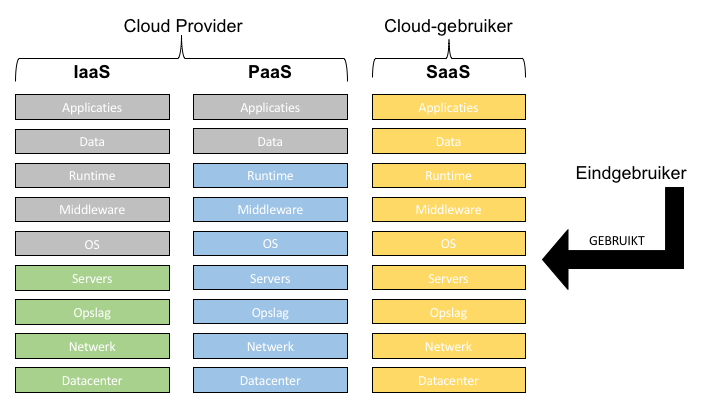
\includegraphics[width=\textwidth]{images/cloud_rollen.png}
	\caption{Image with caption.}
	\label{fig:cloud_rollen}
\end{figure}

Example of a code fragment. Minted supports modern programming languages such as Rust and Golang, and modern configuration formats such as YAML.

\begin{listing}[ht]
\begin{minted}[fontsize=\footnotesize,samepage]{rs}
// This is the main function.
fn main() {
    // Statements here are executed when the compiled binary is called.

    // Print text to the console.
    println!("Hello World!");
}
\end{minted}
\caption{This hello-world code fragment is deceivingly simple. Most rust programs are a lot more difficult to comprehend.}
\end{listing}



\section{Section title}

Table~\ref{tab:resallocschemes} shows an overview of..

\begin{table}[h]
	\centering
	\captionsetup{justification=centering}
	\caption[Overzicht resource-allocatieschema's]{Overzicht resource-allocatieschema's}
	\label{tab:resallocschemes}
	\resizebox{\textwidth}{!}{%
	\begin{tabular}{L{4cm} l C{2cm} c c c c}
		\toprule
		Naam & Jaar & Type  & A | F | P  & Invoer & Uitvoer & Getest  \\ \midrule
		Alicherry et al.~\cite{Alicherry2012} & 2012 & k-sneden & A & G & par\{G\} & S \\
		MCRVMP~\cite{Biran2012} & 2012 & ILP \& GH & A & B\{netwerk\} & VM-plaatsing & C\\
		\bottomrule
	\end{tabular}}
\end{table}
